\documentclass[usenames,dvipsnames,tikz]{standalone}
%\usepackage{xcolor}
%\definecolor{tLightOrange1}{HTML}{FFCD4F} %tikz color
%\colorlet{tLightGreen}{LimeGreen!70!OliveGreen!30!White}
\definecolor{tLightGreen}{HTML}{D3ECAA}
%\colorlet{tLightOrange}{Dandelion!65!White}
\definecolor{tLightPink}{HTML}{FFD4EB} %tikz color
\definecolor{tLightBlue}{HTML}{CEF0FF} %tikz color
%\usepackage{tikz}
%\usepackage{standalone}
\begin{document}
	
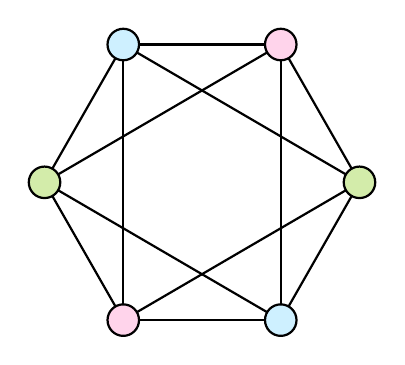
\begin{tikzpicture}
%v1=1, v2=1, v3=2, v4=2, v5=3, v6=4, v7=4, v8=5, v9=5, v10=6, v11=6, v12=6, v13=6, v14=7, v15=8, v16=9
%\draw [help lines] (-1,-1) grid (8, 13);

\draw [thick] (2.5,0) -- (4.5,0);
\draw [thick] (2.5,0) -- (2.5,3.5);
\draw [thick] (2.5,0) -- (1.5,1.75);
\draw [thick] (2.5,0) -- (5.5,1.75);
\draw [thick] (4.5,0) -- (5.5,1.75);
\draw [thick] (4.5,0) -- (4.5,3.5);

\draw [thick] (4.5,0) -- (1.5,1.75);
\draw [thick] (1.5,1.75) -- (2.5,3.5);
\draw [thick] (2.5,3.5) -- (5.5,1.75);
\draw [thick] (2.5,3.5) -- (4.5,3.5);
\draw [thick] (5.5,1.75) -- (4.5,3.5);
\draw [thick] (4.5,3.5) -- (1.5,1.75);


%C1 - vertices
\draw [fill=tLightPink, thick] (2.5,0) circle [radius = 0.2]; % bottom left
\draw [fill=tLightBlue, thick] (4.5,0) circle [radius = 0.2]; % bottom right
\draw [fill=tLightGreen, thick] (1.5,1.75) circle [radius = 0.2]; % middle left
\draw [fill=tLightGreen, thick] (5.5,1.75) circle [radius = 0.2]; % middle right
\draw [fill=tLightBlue, thick] (2.5,3.5) circle [radius = 0.2]; % top left
\draw [fill=tLightPink, thick] (4.5,3.5) circle [radius = 0.2]; % top right





\end{tikzpicture}
	
\end{document}
